\documentclass[]{article}
\usepackage{JML}
\usepackage{amsfonts}
\usepackage{graphicx}
\usepackage{dsfont}
\usepackage[left=1in,right=1in]{geometry}
\title{The CLP: Constrained Linear Predictors}
\setlength\parskip{5pt}
\setlength\parindent{0pt}
\def\llangle{\left\langle}
\def\rrangle{\right\rangle}
\newcommand\E[1]{\llangle #1 \rrangle}
\newcommand\T[1][i]{\mathcal{T}_{#1}}
\def\a{\vec{a}_t}
\def\ai{\vec{a}_{t_i}}
\def\vi{\vec{v}_i}
\def\wi{\vec{w}}
		
\begin{document}
	\maketitle

	\section*{The Goal}
		Consider a second order random process $X$, such that at each value of $t \in \mathbb{R}$, we have a random variable $X_t$. 

		We may randomly sample this vector at $n$ points, gaining a vector $\vec{T} = (t_1,t_2,t_3,\hdots)$ of times at which the samples were made, and $\vec{X} = (X_{t_i})$. Strictly speaking these are both random variables in and of themselves, up until the moment that we `realise' them. We can index into these vectors using the the integer $0 \leq i < n$, and we assume without loss of generality that the samples are sorted in time, such that $t_i < t_{i+1} \forall i$.

		In the case of the BLP, we wish to find a predictor, $\hat{X}_t$, which will predict the values of $X_t$ on a set of `prediction points', $t \in T$, subject to three further conditions:
		\begin{itemize}
			\item We are willing to present an \textit{a priori} guess at the functional form of the predictor, in the form of a `prior function' $g(t)$.
			\item The only thing we `know' (or are willing to \textit{ansatz}) about $X_t$ is the second moment kernel (a generalisation of the covariance):
			$$ \E{(X_t-g(t)) (X_s-g(s))} = k(t,s)$$
			\item Our predictor should be linear, such that:
			$$\hat{X}_t = g(t) + \vec{a}_t \cdot \left(\vec{X} - \vec{G}\right)$$
			Where $G_i = g(t_i)$
		\end{itemize}
		We again reiterate that $X_t, \vec{X}$ and $\hat{X}_t$ are - strictly speaking - random variables until we make them into real numbers at the moment we wish to actually make a prediction. $\vec{a}_t$ is a real $n$-tuple, which takes on different values at each value of $t$.

		These are the ingredients of the standard BLP. The goal of this work is to extend this by adding one further condition:
		\begin{itemize}
			\item The Predictor should obey a number of constraints of the form $h(\{X_t\}) = 0$
		\end{itemize}
		We are therefore attempting to formulate the \textit{Constrained Linear Predictor} (CLP)
	\section{Deriving the CLP}

		We define the CLP as the linear predictor which minimises the Mean Squared Error, averaged across all realisations of the random variable, computed at the set $T$ of points at which we wish to make predictions, and which obeys our constraints.

		Therefore, the CLP minimises the following Lagrangian:
		\begin{spalign}
			\mathcal{L} & = \sum_{t \in T} \langle (X_t - \hat{X}_t)^2 \rangle - \sum_j \lambda_j h_j(\{\hat{X}\}) \label{E:GlobalLagrangian}
		\end{spalign}
		Here $h_j(\{\hat{X}_t\})$ is the $j^\text{th}$ constraint on the \textit{prediction points}\footnote{For clarity and avoidance of symbol-collision with the other X-s, we will denote the prediction points as $P_i = \hat{X}_{t_i} = g(t_i) + \a \cdot \vec{X}^\prime$}, such that $h_j = 0$ when the constraint is met, and is non-zero otherwise, with the sum running over all such constraints. $\lambda_j \in \mathbb{R}$ are the associated Lagrange Multipliers. In the standard BLP we are able to treat the Lagrangian as separable in each element of $T$ - minimising the MSE individually at each $t\in T$ is equivalent to performing a global minimisation: in the CLP this is not true, and we must consider the global case.

		The issue at present is that we do not know what the behaviour of $X_t$ is -- we might have an initial guess (i.e. our prior, $g(t)$), but the entire purpose of this exercise is that we do not know $X_t$. However, by expanding out the brackets, we are able to write the Lagrangian in the following form:
		\begin{spalign}
			\mathcal{L} & = \left[\sum_{t \in T} \E{{X_t^\prime}^2} - 2\a  \cdot \E{X_t^\prime \vec{X}^\prime} + \E{(\a \cdot \vec{X}^\prime)^2} \right] - \sum_j \lambda_j h_j(\{\hat{X}\})
			\\
			& = \left[\sum_{t \in T} \E{{X_t^\prime}^2} - 2\a  \cdot \vec{k}_t + \a \cdot (K \a) \right] - \sum_j \lambda_j h_j(\{\hat{X}\})
		\end{spalign}
		Where:
		\begin{spalign}
			X_t^\prime & = X_t - g(t)
			\\
			\vec{X}^\prime & = \vec{X} - \vec{G}
			\\
			\vec{k}_t & \in \mathbb{R}^n \text{ such that } \left[ \vec{k}_t \right]_i = k(t,t_i)
			\\
			K & \in \mathbb{R}^{n\times n} \text{ such that } K_{ij} = k(t_i,t_j)
		\end{spalign}
		Note that since the kernel is, by definition, symmetric in its arguments, $K^T = K$. Note that we have also taken the explicit step of writing our kernel as a relationship between the \textit{transformed} data - i.e. $X^\prime$ - the imposition of different functions $g(t)$ might therefore warrant different kernels. This is true even if the transform is the (commonly used) constant `mean scaling', $g(t) = \E{X_t} \approx \frac{1}{n} \vec{X} \cdot \mathds{1}$.

		By performing this transform we have placed the incomputable terms - that of $\E{(X_t^\prime)^2}$ into a constant term. Since Lagrangians are invariant under constant scalings, it is possible to find an optimal value of $\a$ using only the remaining computable terms. 

		However - as we shall see - we are in the uncomfortable position of trying to impose conditions on the predicted values, $P_i = \hat{X}_{t_i} = g(t_i) + \ai \cdot \vec{X}^\prime$ whilst our object of interest is now the vector $\ai$. 

		We therefore limit ourselves to the case of \textit{linear constraints}, i.e., those which can be written in the following form:
		\begin{spalign}
			h_j(\{P\}) & = c_j - \sum_k d_{jk} P_k
			\\
			& = c_j - \sum_k d_{jk} \left( g(t_k) + \vec{a}_{t_k} \cdot \vec{X}^\prime\right) \label{E:Constraint}
		\end{spalign}
		We can then take the derivative of the Lagrangian with respect to $\ai$, and find that:
		\begin{spalign}
			\pdiv{\mathcal{L}}{\ai} & = 2 K \ai - 2 \vec{k}_i - \sum_j \lambda_j \pdiv{h_j}{\ai}
			\\
			& = 2 K \ai - 2 \vec{k}_i + \left(\sum_j \lambda_j b_{ji}\right) \vec{X}^\prime
			\\
			& = 2 K \ai - 2 \vec{k}_i + \eta_{i} \vec{X}^\prime
		\end{spalign}
		Hence, the optimal value of $\ai$ is:
		\begin{spalign}
			\ai & = K^{-1} \left( \vec{k}_i - \frac{\eta_i}{2} \vec{X}^\prime \right)
			\\
			& = \vi - \frac{\eta_i}{2} \wi
		\end{spalign}
		The optimal predicted value is:
		\begin{spalign}
			P_i & = g(t_i) + \ai \cdot \vec{X}^\prime
			\\
			& = g(t_i) + \vi \cdot \vec{X}^\prime - \frac{\eta_i}{2} \wi \cdot \vec{X}^\prime
			\\
			& = g(t_i) + A_i - \frac{\eta_i}{2} B \label{E:LagrangeOptim}
		\end{spalign}

		\subsection{Exact Constraints}

			In the case where the constraints $h_j$ are exact -- i.e. the sets $\{c\}$ and $\{d\}$ are exactly determined, we may therefore analytically solve to find the set of Lagrange multipliers, then $\vec{\eta}$, and hence compute the predictor. We note that $\vec{\eta}$ can be written as:
			\begin{equation}
				\vec{\eta} = D^T \vec{\lambda}
			\end{equation}
			Where $D_{ij} = d_{ij}$ is the constraint matrix, $\vec{\eta}_k = \eta_k$ is a vector on $\mathbb{R}^N$ and $\vec{\lambda}_k = \lambda_k$ is a vector on $\mathbb{R}^m$, where $m$ is the number of constraints. The requirement that the constraints are met can be written as:
			\begin{spalign}
				D \vec{p} = \vec{c}
			\end{spalign} 
			Where $\vec{p}_i = P_i$ is another vector on $\mathbb{R}^n$ and $\vec{c}_i = c_i \in \mathbb{R}^m$. Writing $g(t_i) + A_i = q_i$, this is then:
			\begin{spalign}
				D\left(\vec{q} - \frac{B}{2} D^T \vec{\lambda} \right) = \vec{c} \LLR \vec{\lambda} = \frac{2}{B} \left(D D^T \right)^{-1} \left( D \vec{q} - \vec{c} \right)
			\end{spalign}
			Therefore:
			\begin{spalign}
				\vec{p} =  \left( \mathds{1}_N - D^T (D D^T)^{-1} D\right)\vec{q} + D^T (DD^T)^{-1} \vec{c} \label{E:ConstrainedSolution}
			\end{spalign}
			In the case where there is only a single constraint ($m=1$), this simplifies such that $D \to \vec{d}^T$:
			\begin{spalign}
				\vec{p} = \vec{q} + \frac{c - \vec{q}\cdot \vec{d}}{\vec{d}^2} \vec{d} 
			\end{spalign}
			% \subsubsection*{An Example}
			% 	Consider the case of two constraints: the fucntion must integrate to some value ($\mathcal{I}$), and the prediction is fixed at some known value for a given $\ell$, such that $P_\ell = \mathcal{P}$.

			% 	This gives:
			% 	\begin{spalign}
			% 		D_{ij} & = \begin{cases} 1 & i = 0 \text{ or } j 0 \ell
			% 			\\
			% 			0 & \text{else}
			% 		\end{cases}
			% 		\LLR D \in \mathbb{R}^{2\times N}
			% 		\\
			% 		\vec{c} & = \begin{pmatrix} \mathcal{I} \\ \mathcal{P} \end{pmatrix}
			% 	\end{spalign}
			% 	Therefore:
			% 	\begin{spalign}
			% 		D^T D = \begin{pmatrix}
			% 			N & 1
			% 			\\
			% 			1 & 1
			% 		\end{pmatrix} \LLR (D^T D)^{-1} = \frac{1}{N-1} \begin{pmatrix} 1 & -1 \\ -1 & N \end{pmatrix}
			% 	\end{spalign}
		\subsection{Inexact Constraints}

			In the case where the constraints are not exact, but serve to enforce bounds -- i.e. monotonicity or positivity -- there is a problem since the parameters of the constraint are not fixed. We may not care, for example, how much greater $X_{i+1}$ is than $X_i$ is, only that it \textit{is} greater. 

			We could enforce this through slack variables and utilise the KKT conditions, however for our purposes it is better to \textit{parameterise} the constraint. 

			Various parameterisations are possible, but perhaps the most comprehensible is to consider that the \textit{prediction} points, $P_i$ are a function of some other parameters $\vec{\theta} \in R^m$, such that:
			\begin{spalign}
				P_i & = \T(\vec{\theta})
				\\
				h_j(\T(\vec{\theta})) &= 0 ~\forall~i,j, \vec{\theta}
			\end{spalign}
			For example, in the case of enforcing positivity, we might have that $P_i = e^{z_i}$, which is equivalent to asserting that $d_{ij} = \delta_{ij}$ and $c_i = e^{z_i}$. Rearranging \eref{E:LagrangeOptim}, we are able to write $\eta_i$ as a function of this Transform, and hence write $\ai$ in the following form:
			\begin{spalign}
				\ai = \vi + \frac{P_i(\vec{\theta}) - A_i - g(t_i)}{B} \wi \label{E:Reparam}
			\end{spalign}
			This might seem somewhat tautological - we have written $\ai$ in terms of the prediction values - but the entire purpose of $\ai$ is to make predictions!

			The usefulness of this comes evident when we insert \eref{E:Reparam} back into the Lagrangian -- essentially performing a change of coordinates from $\mathcal{L}(\vec{a},\vec{\theta})$ to $\mathcal{L}(\vec{\theta})$, since we have now ensured that $\a$ will always be at its optimal value for each value of $\vec{\theta}$. 
			\begin{align}
				\vec{k}_i \cdot \ai & = \vi \cdot \vec{k}_i + \frac{P_i(\vec{\theta}) - A_i - g(t_i)}{B} \wi \cdot \vec{k}_i
				\\
				\begin{split}
					~
					\\
				\ai \cdot (K\ai) & = \left(\vi + \frac{P_i(\vec{\theta}) - A_i - g(t_i)}{B} \wi  \right) \cdot\left(\vec{k}_i + \frac{P_i(\vec{\theta}) - A_i - g(t_i)}{B} \vec{X}^\prime  \right) 
				\\
				& =  \vi \cdot \vec{k}_i + \left(\frac{P_i(\vec{\theta}) - A_i - g(t_i)}{B}\right)\left(\wi \cdot \vec{k}_i + A_i\right) + \frac{\left(P_i(\vec{\theta}) - A_i - g(t_i)\right)^2}{B}
				\end{split}
			\end{align}
			Since $\vec{w} \cdot \vec{k}_i = (K^{-1} \vec{X}^\prime) \vec{k}_i = (K^{-1} \vec{k}_i) \vec{X}_\prime = \vi \cdot \vec{X}^\prime = A_i$ due to the symmetry of $K$, and the constraints are all automatically satisfied thanks to our parameterisation, we find that the Lagrangian simplifies to:
			\begin{spalign}
				\mathcal{L}(\vec{\theta}) & =  \sum_i \left( \E{(X_i^\prime)^2} -   \vec{k}_i \cdot \vi \right) + \frac{1}{B} \left(P_i(\theta) - A_i - g(t_i)\right)^2
				\\
				& =  \text{const in $\vec{\theta}$} + \frac{1}{B}\sum_i\left(P_i(\theta) - A_i - g(t_i)\right)^2
				\\
				\mathcal{L}^\prime & = \sum_i P_i\left(P_i(\theta) - 2 (A_i + g(t_i))\right)
			\end{spalign}
			Where in the final line we took the opportunity to perform a rescaling (recalling that $B > 0$ is enforced by the positive definiteness of $K$) which leaves the optimum invariant. In some cases it is trivial to identify the optimal values of $P_i$ - for example, in the case where $P_i = e^{\theta_i}$, the maximum is evidently:
			\begin{equation}
				P_i = \begin{cases} A_i + g(t_i) & \text{if this is } > 0
					\\
					0 & \text{else}
				\end{cases}
			\end{equation}
			In short, the CLP is equal to the BLP except when the condition is violated, at which point a hard cut is placed on it. 

			More complex conditions however, can lead to more complex behaviour - the monotonicity constraint, for example, exhibits the obvious behaviour that it again follows the BLP when it is monotonic, and is flat when the BLP has a negative gradient -- but the \textit{location} where the CLP becomes flat is non-trivial, with flatness necessarily occuring \textit{before} the BLP changes direction: a tradeoff in following the BLP locally versus becoming too large too early without the ability to decrease due to the monotonic constraint.

			In these cases a more complex search is required -- where the behaviour of the constraint is evident \textit{a priori} (such as the monotonic constraint), one can limit the space of the search. In the general case, however, a numerical optimisation is required. 

			The derivative of the Lagrangian with respect to the constraint parameters is:
			\begin{spalign}
				\pdiv{\mathcal{L}^\prime}{\theta_m} = 2\sum_i \left(P_i - A_i - g(t_i)\right) \pdiv{P_i}{\theta_m}
			\end{spalign}
			This can be used to numerically optimise the values of $\vec{\theta}$

		\subsection{Inexact Constraints (Redux)}
			
			We note that we performed a fairly drastic change in approach between the exact constraints and the inexact constraints -- is it possible to maintain the same approach for both?

			We consider now that the parameters $\vec{c}$ of the constraints are functions of an (unconstrained) external parameter, $\vec{z} \in \mathbb{R}^m$ - letting $\vec{c} = \text{const}$ recovers the condition of the exact equalities. However, in any  other case we must still find the values of $\vec{z}$ which optimise the global Lagrangian - and hence we need to rewrite our Lagrangrian in terms of $\vec{c}$.

			From \eref{E:ConstrainedSolution}, we can rewrite the predicted value-vector (recalling that $\vec{p}_i = P_i = \hat{X}_{t_i}$) as:
			\begin{spalign}
				\vec{p} & = \vec{j} + R \vec{c}(\vec{z})
				\\
				R &= D^T (D D^T)^{-1}
				\\
				\vec{j} = \left( \mathds{1}_N - R D\right) \vec{q} &\LLR j_i  = g(t_i) + A_i + \sum_{j,k} R_{ij}D_{jk} (g(t_k) + A_k)%\left( \mathds{1}_N - D^T (D D^T)^{-1} D\right) \left(	
			\end{spalign}
			We note that from a conceptual standpoint it is not a problem for the `mixing' constraints $D_{ij}$ to be the functions of $\vec{z}$, but this assumption allows us to precompute many of the otherwise troublesome entities. We can also rewrite $\ai$ as:
			\begin{spalign}
				\ai & = \vi - \frac{\eta_i}{2} \wi
				\\
				& = \vi +  \frac{\left[R\left(\vec{c} - D \vec{q}  \right) \right] \cdot \hat{e}_i}{B} \wi
				\\
				& = \vec{j}_i + \frac{(R\vec{c})\cdot \hat{e}_i}{B} \wi
			\end{spalign}
			Where
			\begin{spalign}
				R&= D^T (D D^T)^{-1}
				\\
				\vec{j}_i & = \vi - \frac{(RD\vec{q})\cdot\hat{e}_i}{B}\wi
			\end{spalign}
			We therefore have:
			\begin{spalign}
				\vec{k}_i \cdot \ai & = \vi \cdot \vec{k}_i + \frac{A_i}{B} \left((R\vec{c}) \cdot\hat{e}_i - (RD\vec{q})\cdot \hat{e}_i\right)
				\\
				&= \text{const in $\vec{c}$} + \frac{A_i}{B} (R \vec{c})\cdot \hat{e}_i
				\\
				\ai \cdot \left(K\ai\right) & = \left(\vec{j}_i + \frac{(R\vec{c})\cdot \hat{e}_i}{B} \wi \right) \cdot  \left(K\vec{j}_i + \frac{(R\vec{c})\cdot \hat{e}_i}{B} \vec{X} \right)
				\\
				& = \text{const in $\vec{c}$} + 2\frac{(R\vec{c})\cdot \hat{e}_i}{B} \vec{j}_i \cdot \vec{X} + \frac{1}{B}((R \vec{c}) \cdot \hat{e}_i)^2
				\\
				& = \text{const in $\vec{c}$} + 2\frac{(R\vec{c})\cdot \hat{e}_i}{B}\left(A_i - (RD\vec{q})\cdot\hat{e}_i\right)  + \frac{1}{B}((R \vec{c}) \cdot \hat{e}_i)^2
			\end{spalign}
			Therefore:
			\begin{spalign}
				\mathcal{L}^\prime & = \sum_i \ai \cdot K\ai - 2 \vec{k}_i \cdot \ai 
				\\
				& = \text{const in $\vec{c}$} + \sum_i ((R \vec{c}) \cdot \hat{e}_i)^2 - 2(R\vec{c})\cdot \hat{e}_i(RD\vec{q})\cdot\hat{e}_i
				\\
				& = \text{const in $\vec{c}$} + (R \vec{c})^2 - 2 (R \vec{c})\cdot(RD\vec{q})
				\\
				& = \text{const in $\vec{c}$} + \left( R \vec{c}(\vec{z}) - RD \vec{q} \right)^2
			\end{spalign}
			The derivative with respect to the (unconstrained) vectors $\vec{z}$ is:
			\begin{spalign}
				\pdiv{\mathcal{L}^\prime}{z_m} & = \left( R \vec{c}(\vec{z}) - RD \vec{q} \right) \cdot R \pdiv{\vec{c}}{z_m}
				\\
				& = \left( \vec{p}(\vec{z}) - \vec{q} \right) \cdot R \pdiv{\vec{c}}{z_m}
			\end{spalign}
			Since $\vec{q}$ is the BLP prediction we can once again see that the derivative is zero if the BLP obeys the constraints ($\vec{c} - D \vec{q} = 0$), so the CLP will always revert to the BLP if this meets our constraints. 
		% \subsection{Mixed Constraints}

		% 	We now consider the case where some of our constraints are exact equality constraints, whilst others are inequality constraints. We denote the equality constraints as $e(\{P\})$, and the inequality constraints as $m(\{P\})$. 

		% 	The derivation proceeds exactly as before, but \eref{E:LagrangeOptim} has two terms:
		% 	\begin{spalign}
		% 		P_i &= g(t_i) + A_i - \frac{B}{2} \left( \epsilon_i + \mu_i \right)
		% 		\\
		% 		~
		% 		\\
		% 		\epsilon_i& = \sum_{j \in \text{equality}} \lambda_j b_{ji}
		% 		\\
		% 		\mu_i & = \sum_{j \in \text{inequality}} \lambda_j b_{ji}
		% 	\end{spalign}
		% 	The value of $\vec{\epsilon}$ can be determined in exactly the same way as $\vec{\eta}$ in the pure-equality case:
		% 	\begin{equation}
		% 		\vec{\epsilon} = (D_e^T D_e)^{-1} D_e^T \vec{r}_e
		% 	\end{equation}
		% 	Where $D_e$ is the constraint matrix derived from the equality subset $\{e_j\}$, and so on.
	\section{The CLUP}

		In the prior work, we assumed the the function $g(t)$ was `handed down' to us to act as a prior function. However, this may induce biases in our predictor, meaning that:
		\begin{equation}
			\E{X_t - \hat{X}_t} \neq 0
		\end{equation}
		We should ideally search for an \textit{unbiased} predictor. The derivation of the Constrained Linear Unbiased Predictor (CLUP) should follow along similar lines to the standard BLUP, but we reproduce it in full for the sake of rigour. 

		We suppose that our random variable $X_t$ can be written as:
		\begin{equation}
			X_t = m(t) + Y_t
		\end{equation}
		Where $m:R \to R$ is the `mean function' and $Y_t$ is a zero-mean random variable. Therefore:
		\begin{equation}
			\E{X_t} = m(t)
		\end{equation}
		The main difference between $m(t)$ and $g(t)$ is that we assumed $g(t)$ was just a prior to `help us along' without any intrinsic relation to $X_t$ -- here, however, we are asserting that $m(t)$ is a meaningful function -- albeit an incomputable one, since we remain unwilling to assert any properties on $\E{X_t}$. Because of this restriction, we cannot subtract away $m(t)$ from our data to formulate $\vec{X}^\prime = \vec{Y}$ -- we must keep everything in terms of our original, untransformed data.

		We \textit{can}, however, assert that $m(t)$ can be decomposed into a sum of basis functions, $\vec{\varphi}(t)$, where $\varphi_i(t): \mathbb{R} \to \mathbb{R}$ is the $i^\text{th}$ basis function. We therefore have:
		\begin{spalign}
			m(t) & = \sum_{i = 0}^\omega \phi_i(t) \beta_i
			\\
			& = \vec{\beta} \cdot \vec{\varphi}(t)
		\end{spalign}
		We again note that $\vec{\beta}$ is not a known value, however, we continue in the expectation that it will cancel out in future. We also note that without further information we must assume that $\omega \to \infty$, in practive we can limit the dimensionality by assuming that $m_\omega(t) \approx m(t)$ for finite $\omega$. We can also formulate the matrix $\Phi$:
		\begin{spalign}
			\Phi \in \mathbb{R}^{\omega\times n} \text{ such that } \Phi_{ij} = \varphi_i(t_j)
		\end{spalign}
		Therefore:
		\begin{spalign}
			\vec{X}_i = \sum_{j}^\omega \Phi_{ji} \beta_j \LLR \vec{X} = \Phi^T \vec{\beta} + \vec{Y}
		\end{spalign}
		
		
		Our linear predictor takes the form:
		\newcommand\vb{\vec{\beta}}
		\begin{spalign}
			\hat{X}_t & = \a \cdot \vec{X}
			\\
			& = \a \cdot (\Phi^T \vb) + \a \cdot \vec{Y}
			\\
			& = \vb \cdot (\Phi \a) + \a \cdot \vec{Y} \label{E:BLUP_X}
		\end{spalign}
		We can also note that:
		\begin{spalign}
			X_t - \hat{X}_t & = \left( \Phi \a - \vec{\varphi}_t \right) \cdot \vb + Y_t - \a \cdot \vec{Y}
		\end{spalign}
		Since $\E{Y} = \vec{0}$ and $\E{Y_t} = 0$ by definition, we note that the unbiased constraint is equal to:
		\begin{spalign}
			\E{X_t - \hat{X}_t} = 0 \LLR \left(\Phi\a - \vec{\varphi}_t\right) \cdot \E{\vec{\beta}} = 0
		\end{spalign}
		Therefore if we write our unbiased constraint as $\mathcal{U}_t = \E{X_t - \hat{X}_t}$, such that $\mathcal{U}_t = 0$ when the constraint is met:
		\begin{spalign}
			\mu_t \mathcal{U}_t & = \left( \mu_t \E{\vec{\beta}} \right) \cdot \left(\Phi\a - \vec{\varphi}_t\right)
			\\
			& = \tilde{\mu}_t \cdot \left(\Phi\a - \vec{\varphi}_t\right)
		\end{spalign}
		A suitable change of coordinates $\mu_t \to \tilde{\mu}_t$ therefore enables us to bypass the unknown $\E{\vec{\beta}}$. Hence the Lagrangian of the system takes the form:
		\begin{spalign}
			\mathcal{L}(\vec{a},\vec{\lambda},\{\tilde{\mu}\}) & = \sum_{t \in T} \left( \E{(X_t - \hat{X}_t)^2} + \tilde{\mu} \cdot \left(\Phi\a - \vec{\varphi}\right) \right)+ \sum_j \lambda_j h_j(\{\hat{X}\})
			\\
			& = \sum_{t \in T} \left(\E{X_t^2} + \a \cdot (K \a) - 2 \vec{k}_t \cdot \a + \tilde{\mu} \cdot \left(\Phi\a - \vec{\varphi}\right) \right)+ \sum_j \lambda_j h_j(\{\hat{X}\})
		\end{spalign}
		This is identical in form to \eref{E:LagrangeOptim}, with the addition of some additional constraints - those labelled by $\tilde{\mu}$, which act to ensure that $\E{X_t - \hat{X}_t} = 0$ for all $t\in T$, i.e. we are now including \textit{unbiasedness} as a constraint.

		We have also introduced $\vec{k}_t$ and $K$ as the second moment matrices on $X$:
		\begin{spalign}
			K \in \mathbb{R}^{n\times n} ~~~~&~~~~ K_{ij} = \E{X_{t_i} X_{t_j}}
			\\
			\vec{k}_t \in \mathbb{R}^n ~~~~&~~~~[\vec{k}_t]_i = \E{X_t X_{t_i}}
		\end{spalign}
		We once again impose the linearity condition on our constraints, such that $h_j = c_j - \sum_k d_{jk} \hat{X}_{t_k}$:
		\begin{spalign}
			\vec{h} = \vec{c} - D \vec{p}
		\end{spalign}
		Where $\vec{p}_i = \hat{X}_{t_i}$. The Lagrangian therefore simplifies to:
		\begin{spalign}
			\mathcal{L}(\vec{a},\vec{\lambda},\{\tilde{\mu}\},\vec{c})& = \sum_{t \in T} \left(\E{X_t^2} + \a \cdot (K \a) - 2 \vec{k}_t \cdot \a + \tilde{\mu} \cdot \left(\Phi\a - \vec{\varphi}_t\right) \right)+ \vec{\lambda} \cdot \left( \vec{c} - D \vec{p} \right)
		\end{spalign}
		The Lagrangian derivatives are:
		\begin{align}
			\begin{split}
			\pdiv{\mathcal{L}}{\ai} & = 2 K \ai - 2 \vec{k}_i + \Phi^T \tilde{\mu} +   \pdiv{\vec{p}}{\ai}(D^T\lambda)
			\\
			& = 2 K \ai - 2  \vec{k}_i + \Phi^T \tilde{\mu} + Q_i(\vec{X}) D^T\vec{\lambda}
			\end{split}
			\\\label{E:CLUP_Constraint}
			\pdiv{\mathcal{L}}{\vec{\lambda}} & =\vec{c} - D\vec{p}
			\\
			\pdiv{\mathcal{L}}{\tilde{\mu}} & = \Phi_t \a - \vec{\varphi}_t \label{E:CLUP_Unbiased}
		\end{align}
		Where $Q_i(\vec{X})\vec{v} = \vec{v} \cdot \hat{e}_i \vec{X}$, and equivalently $Q_i^T \vec{v} = \vec{v} \cdot \vec{X} \hat{e}_i$, where $\hat{e}_i$ is the $i^\text{th}$ basis vector, such that $\vec{\lambda} \cdot \hat{e}_i = \lambda_i$, the $i^\text{th}$ Lagrange Multiplier \footnote{We note that we are having something of a collision with vectors associated with the $i^\text{th}$ predictor (such as $\ai$) and scalars associated with predictors or constraints which we have `stacked' into vectors - such as $\lambda_i$ and $P_i$. When indexing into labelled vectors we will attempt to make this clear - i.e. $[\ai]_j$ is the $j^\text{th}$ element of the vector associated with predictor $i$}.	The optimal value of $\a$ is therefore at:
		\def\vl{\vec{\lambda}}
		\begin{spalign}
			\ai & = K^{-1} \vec{k}_i - 2 K^{-1} \Phi^T \tilde{\mu}_i + K^{-1} Q_i D^T \vec{\lambda}
			\\
			& = \vi - 2 K^{-1}\Phi^T \tilde{\mu}_i + (D^T \vl) \cdot \hat{e}_i \wi \label{E:CLUP_a}
		\end{spalign}

		\subsection{Applying Constraints}
			We now impose the unbiased constraint - substituting \eref{E:CLUP_a} into \eref{E:CLUP_Unbiased}, which gives us:
			\begin{spalign}
				\Phi \vi - 2 \Phi K^{-1} \Phi^T \tilde{\mu}_i + (D^T \vl) \cdot \hat{e}_i \Phi_t \wi = \vec{\varphi}_i
			\end{spalign}
			Here we have again switched notation to $\vec{\varphi}_i = \vec{\varphi}_{t_i}$ for convenience. Solving for $\tilde{\mu}_i$:
			\begin{spalign}
				\tilde{\mu}_i & = \frac{1}{2} \left(\Phi K^{-1} \Phi^T\right)^{-1} \left( \Phi \vi + (D^T \vl) \cdot \hat{e}_i \Phi_t \wi - \vec{\varphi}_i\right)
				\\
				& = \frac{1}{2}{M}^{-1} \left( \Phi \vi + (D^T \vl) \cdot \hat{e}_i \Phi_t \wi - \vec{\varphi}_i\right)
			\end{spalign}
			And therefore
			\begin{spalign}
				\ai & = \left(\mathds{1} - K^{-1} \Phi^T{M}^{-1}\Phi \right)\vi +K^{-1} \Phi^T {M}^{-1} \vec{\varphi}_i + (D^T \vl) \cdot \hat{e}_i \left(\mathds{1} - K^{-1} \Phi^T {M}^{-1} \Phi \right)\wi 
				\\
				& = B \vi + C \vec{\varphi}_i + (D^T \vl) \cdot \hat{e}_i B^i \wi
				\\
				~
				\\
				& \text{where } C = K^{-1} \Phi^T{M}^{-1}
				\\
				& \text{and } B =  \left(\mathds{1} - C \Phi \right)
			\end{spalign}

			The prediction values are therefore:
			\begin{spalign}
				\hat{X}_i = P_i & = \ai \cdot \vec{X}
				\\
				& = (B{\vi} + C \vec{\varphi}_i)\cdot \vec{X} + (D^T \vl) \cdot \hat{e}_i \vec{X} \cdot B K^{-1} \vec{X}
				\\
				& = \alpha_i + (D^T \vl) \cdot \hat{e}_i \beta
			\end{spalign}
			Where $\alpha_i$ and $\beta_i$ are generalisations of the $A_i$ and $B_i$ terms used in the CLP. We can then form a vector of $\vec{p}_i = P_i$, such that:
			\begin{spalign}
				\vec{p} & = \vec{\alpha} + \beta D^T \vl
			\end{spalign}
			Inserting this into the imposed constraints of \eref{E:CLUP_Constraint}, we find:
			\begin{spalign}
				D \vec{p} & = \vec{c}
				\\
				D \vec{\alpha} + \beta D D^T \vl= \vec{c}
				\\
				\vl & = \frac{1}{\beta}\left(D D^T \right)^{-1} \left(\vec{c} - D \vec{\alpha}\right)
			\end{spalign}

		\subsection{The CLUP}
			We can then insert this back into the definition of $\ai$ to find:
			\begin{spalign}
				\ai^\text{clup} &= B \vi + C \vec{\varphi}_i + \frac{\left(D^T \left(D D^T \right)^{-1} \left(\vec{c} - D A^\text{blup}\vec{X}\right)\right)\cdot \hat{e}_i}{\beta} B K^{-1} \vec{X}
				\\
				& = \ai^\text{blup} + \frac{\left(D^T \left(D D^T \right)^{-1} \left(\vec{c} - D A^\text{clup}\vec{X}\right)\right)\cdot \hat{e}_i}{\beta} B K^{-1} \vec{X}
			\end{spalign}
			Where:
			\begin{spalign}
				C & = K^{-1} \Phi^T  (\Phi K^{-1} \Phi^T)^{-1}
				\\
				B & = \mathds{1} - C \Phi
				\\
				\beta & = \vec{X} \cdot B K^{-1} \vec{X}
				\\
				\ai^\text{blp} & = K^{-1} \vec{k}_i
				\\
				\ai^\text{blup} & = B \ai^\text{blp} + C\vec{\varphi}_i
				\\
				[A^\text{blup}]_{ij} & = [\ai^\text{blup}]_j
			\end{spalign}

			We reformulate our Lagrangian in terms of $\vec{c}$ in order to allow us to optimise w.r.t. to inexact constraints. For convenience, we write the matrix product as $H = \frac{1}{\beta}D^T(D D^T)^{-1}$. After much algebra, it becomes clear that we can write the Lagrangian in the following form:
			\begin{spalign}
				\mathcal{L}^\prime = \text{constant in $\vec{c}$ } + \left(H\vec{c} - H D \vec{\alpha} + \vec{\ell}\right)^2
			\end{spalign}
			Where:
			\begin{spalign}
				\ell_i & =  \beta\left( {\ai^\text{blup}\cdot \left(KBK^{-1}\right)\vec{X} - \vec{k}_i \cdot B K^{-1} \vec{X}}\right)
			\end{spalign}
			
			% \begin{spalign}
			% 	\vec{k}_i \cdot \ai & = \vec{k}_i \cdot \left(B^i \vi + C \vec{\varphi}_i \right) + \left(H\vec{c} - H D \vec{\alpha} \right)\cdot \hat{e}_i \vec{k} \cdot B^i \vec{w}
			% 	\\
			% 	\ai \cdot K \ai &  = \left(B^i \vi + C \vec{\varphi}_i \right) \cdot K \left(B^i \vi + C \vec{\varphi}_i \right) 
			% 	\\
			% 	& ~~+ 2\left(H\vec{c} - H D \vec{\alpha} \right) \cdot \hat{e}_i ~ \times \wi^T B^i K\left(B^i \vi + C \vec{\varphi}_i \right)
			% 	\\
			% 	& ~~ + \left(\left(H\vec{c} - H D \vec{\alpha} \right) \cdot \hat{e}_i\right)^2 \vec{w}^T B^i K B^i \vec{w}
			% \end{spalign}
			% Therefore:
			% \begin{spalign}
			% 	\ai \cdot K \ai - 2\ai \cdot{\vec{k}} & =\left(\vec{w}^T B^i K B^i \vec{w}\right) \left(\left(H\vec{c} - H D \vec{\alpha} \right) \cdot \hat{e}_i\right)^2 
			% 	\\
			% 	& + 2\left(\left(H\vec{c} - H D \vec{\alpha} \right) \cdot \hat{e}_i\right) \left(\wi^T B^i K\left(B^i \vi + C \vec{\varphi}_i \right) - \vec{k} \cdot B^i \vec{w}\right)
			% \end{spalign}
			As a result, we may write the derivative of the Lagrangian w.r.t. one of the constraint parameters ($\vec{z}_i$) as:
			\begin{spalign}
				\pdiv{\mathcal{L}^\prime}{z_m} & = H^T \left(H(c(\vec{z}) - D\vec{\alpha}) + \vec{\ell} \right) \cdot  \pdiv{\vec{c}}{z_m}
				\\
				& = \left( (DD^T)^{-1} \left[ \vec{c}(\vec{z}) + D\left(\vec{\ell} - \vec{\alpha} \right)\right] \right) \cdot \pdiv{\vec{c}}{z_m}
			\end{spalign}
			In the case where $c_m = f(z_m)$, i.e. each constraint is associated uniquely with a single parameter, this simplifies to:
			\begin{spalign}
				\pdiv{\mathcal{L}^\prime}{\vec{z}} & = \left( (DD^T)^{-1} \left[ \vec{c}(\vec{z}) + D\left(\vec{\ell} - \vec{\alpha} \right)\right] \right) \otimes \vec{\Delta}(\vec{z})
				\\
				~
				\\
				[\vec{\Delta}(\vec{z})]_i & = \left.\pdiv{c_i}{z_i} \right|_{\vec{z}}
			\end{spalign}
			This has the advantage of reducing the number of operations needed to compute the derivative - from $m^2$ to $m$. 
			
	\subsection{The CL(U)P in Action}

		\begin{figure}[t]
			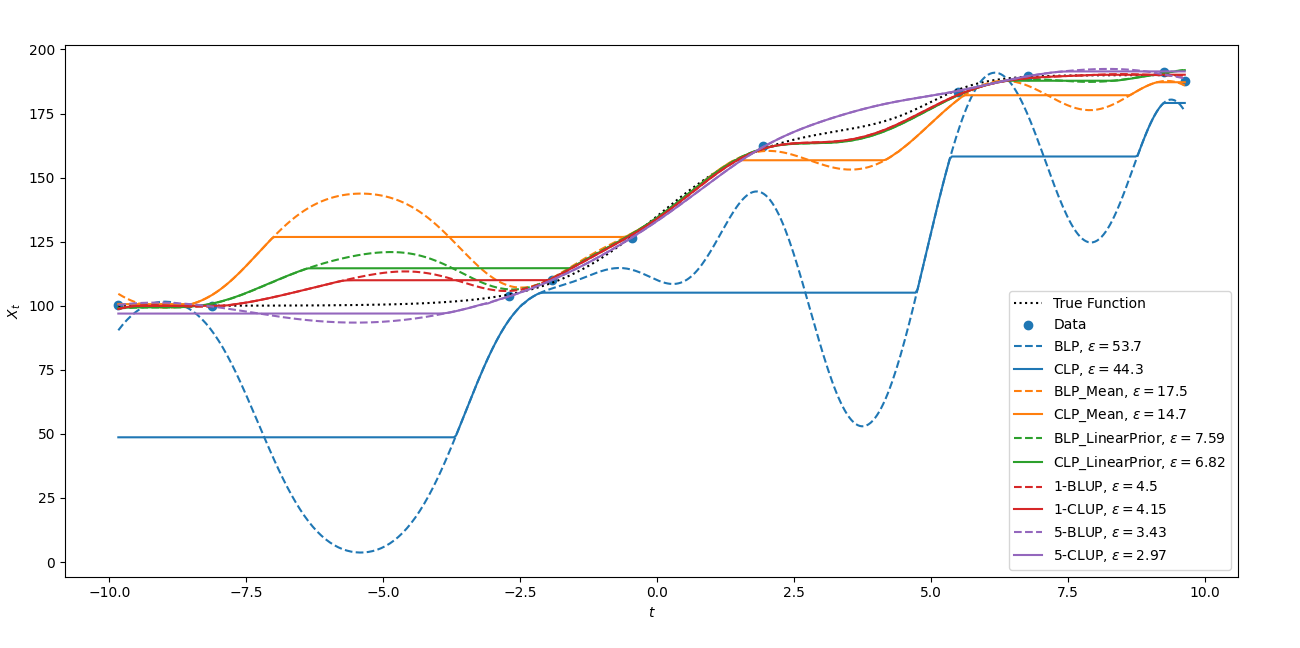
\includegraphics[width=\linewidth,keepaspectratio=true]{Figs/CLUP_comparison.png}
			\caption{\it A series of predictions on a dataset of $N=10$ points drawn from the dotted black curve with Gaussian noise ($\sigma=2$) added on. The models are described in detail in the text. The kernel has is a squared exponential with lengthscale $\ell_0 = 1$ throughout. $\epsilon$ is the RMS deviation from the true, underlying function -- this is distinct from the MSE, which is a function of the data.}\label{F:CLUP}
		\end{figure}

		

		In Figure \ref{F:CLUP}, we show the relative perfomance of the constrained predictors when fitting a bi-sigmoid function with Gaussian noise generated. We impose the constraint that we know the underlying function is \textbf{monotonic}.
		
		The monotonicity constraint means that we should always have $P_{i} \geq P_{i-1}$, assuming the prediction points are suitably time-ordered - our inexact constraint therefore takes the form:
		\begin{spalign}
			\vec{c}(\vec{z}) \in \mathbb{R}^{n-1}~~~&~~~ 	[\vec{c}(\vec{z})]_i = e^{z_i}
			\\
			D \in \mathbb{R}^{(n-1)\times n} ~~~&~~~ D_{ij}  = -\delta_{ij}+ \delta_{(i+1)j}\label{E:CLP_Monotone}
		\end{spalign}

		To our generated dataset, we fitted the following models:
		\begin{itemize}
			\item \textbf{BLP}: A standard BLP using the simple $\vec{X} \cdot K^{-1} \vec{k}$ predictor. We did not perform a mean-scaling on this predictor: $g(t) = 0$.
			\item \textbf{CLP}: As with the BLP, but with the addition of the monotonic constraint (see \eref{E:CLP_Monotone})
			\item \textbf{BLP\_Mean}/\textbf{CLP\_Mean}: As above, but the prior is set to $g(t) = \frac{1}{N} \mathds{1} \cdot \vec{X}$, i.e. the sample mean.
			\item  \textbf{BLP\_LinearPrior}/\textbf{CLP\_LinearPrior}: The prior is set to $g(t) = mt + c$, the straight line joining the two extreme datapoints in the sample. To avoid bootstrapping, these datapoints are then removed from the training dataset, so the fit is performed on $N-2$ datapoints.
			\item $n$-\textbf{BLUP} the standard BLUP, with $\Phi$ expanded to $n^\text{th}$ order. 
			\item $n$-\textbf{CLUP}, as with the $n$-\textbf{BLUP}, but with the addition of the monotonic constraint.
		\end{itemize}

		We note that we deliberately offset and up-scaled the bi-sigmoid to highlight the difficulty faced by the BLP/CLP without the use of a prior function.

		We see this reflected in Fig. \ref{F:CLUP}: the BLP and CLP demonstrate extremely poor fits to the data; with the BLP oscillating down to 0 in the gaps between datapoints. The CLP tries to strike a balance between the BLP fit and remaning monotonic - the result is an underwhelming fit which goes nowhere near the data. 
		
		The addition of a prior $g(t)$ shows a significant improvement in the fit -- the simple mean shift prevents the reversion down to 0, but i.e. at $t \approx -5$ results in a similar deviation upwards. The more complex LinearPrior models show a much better fit - the deviation at $t \approx -5$ is much smaller, and similar improvements are observed at $t \approx3,+7$. This is noteworthy as the model has only 8 points to infer from, and yet shows a better fit than the BLP/CLP\_Mean models which have more data to work from.
		
		The BLUP/CLUP models again show an improvement - the 1-BLUP/1-CLUP models are directly comparable to the LinearPrior models since they both attempt to set a linear function, but the LinearPrior use only the extremum points, and must then remove those datapoints to prevent overfitting: the 1-BLUP and 1-CLUP, however, simultaneously fit the linear fit and the predictor, which gives an improved fit. 

		Finally, the 5-BLUP/5-CLUP models fit a $5^\text{th}$ order polynomial, and demonstrate a significant improvement in the fit -- the model is able to accurately anticipate that the line should be flat at $t\approx-5$.

		We also note that, as measured by the true-RMS ($\epsilon$ in the figure), the inclusion of the monotonic constraint always improved the quality of the prediction -- even the 5-BLUP which provided a good fit was bested by the 5-CLUP, by a non-trivial margin. 

		These conclusions are maintained even as we increase the number of datapoints (as seen in Fig. \ref{F:CLUP2}) -- the margins become notably smaller, which is unsurprising as the predictor will tend towards becoming monotonic even without the inclusion of the constraints, the the CLP/CLUP generally outperform the BLP/BLP even when the amount of data becomes very large - as in Fig. \ref{F:CLUP3}
		\begin{figure}[t]
			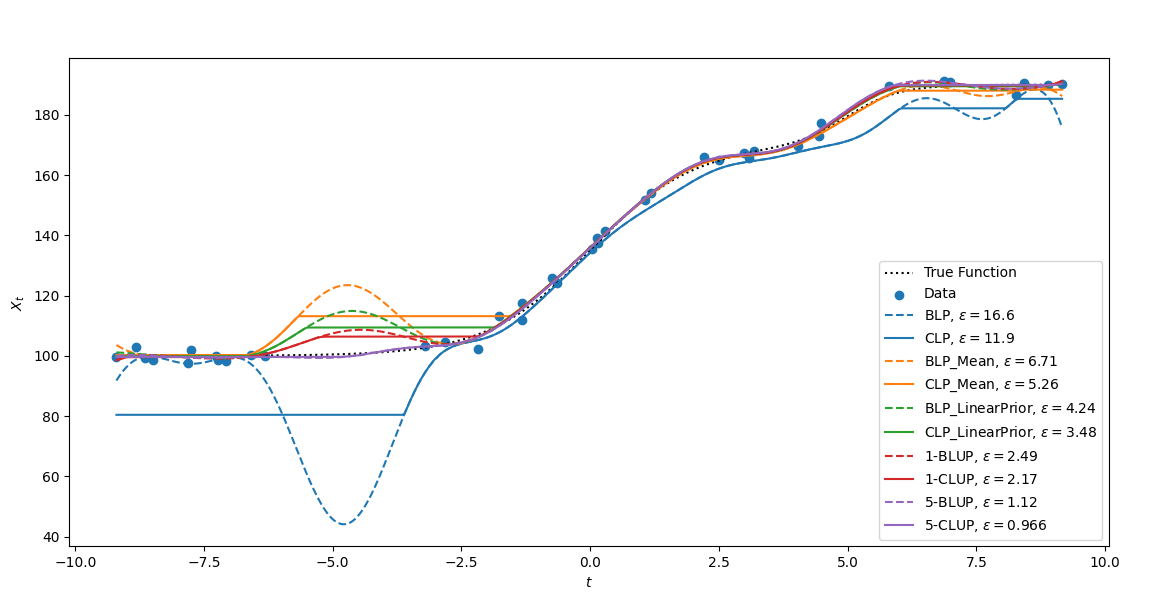
\includegraphics[width=\linewidth,keepaspectratio=true]{Figs/CLUP_comparison_moreData.png}
			\caption{\it As with \ref{F:CLUP}, but with $N=40$ datapoints ($N=38$ for the `Prior' models)}\label{F:CLUP2}
		\end{figure}
		\begin{figure}[t]
			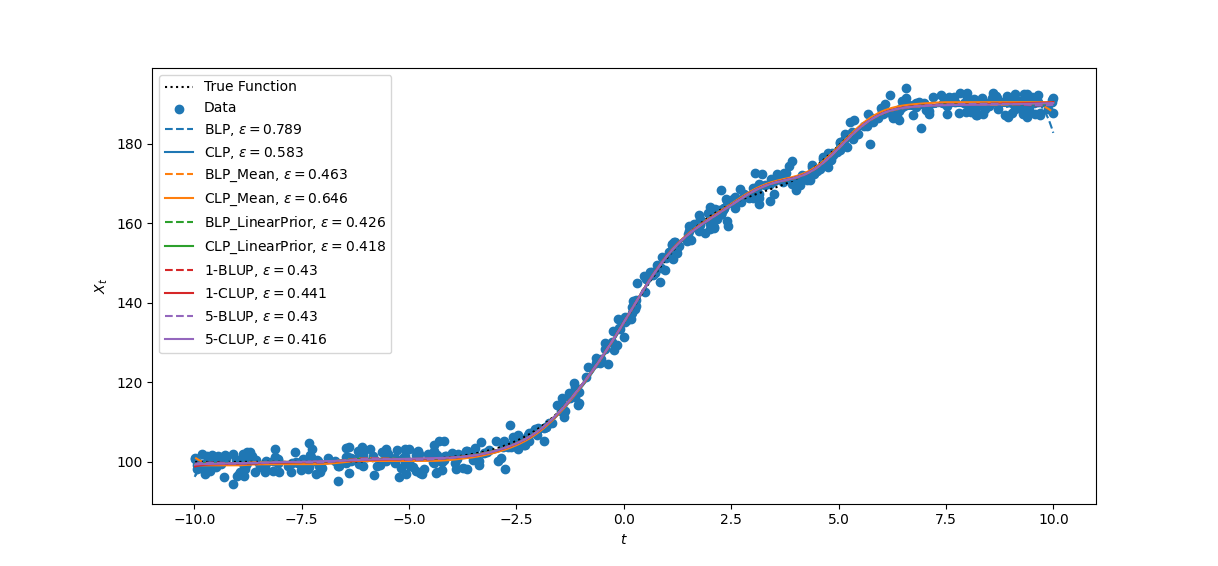
\includegraphics[width=\linewidth,keepaspectratio=true]{Figs/CLUP_comparison_moremoreData.png}
			\caption{\it As with \ref{F:CLUP}, but with $N=520$ datapoints ($N=518$ for the `Prior' models)}\label{F:CLUP3}
		\end{figure}
	\section{Optimising the Kernel}


\end{document}